\documentclass[aspectratio=169]{beamer}
%% AVAILABLE ASPECT RATIOS ARE
%% RATIO | apectratio=
%% 16:10 | 1610
%% 16:9  | 169 % Original PPT theme available in this aspect ratio.
%% 14:9  | 149
%% 5:4   | 54
%% 4:3   | 43 % Original PPT theme available in this aspect ratio.
%% 3:2   | 32

%% THESE PACKAGES ARE JUST FOR THE DEMONSTRATION ---------------------- %%
\usepackage{tikz}
   \usetikzlibrary{matrix}

\newcommand{\key}[1]{\texttt{\color{UOWorange}#1}}
\newcommand{\val}[1]{\texttt{\color{UOWblue}#1}}
\newcommand{\command}[1]{\texttt{\color{UOWdarkgreen}#1}}

\usepackage{metalogo}
\usepackage{chemmacros}
\usepackage{listings}
   \lstset{%
      language=[LaTeX]{TeX},
      basicstyle=\scriptsize\ttfamily,
      keywordstyle=\ttfamily\color{UOWdarkgreen},
      morekeywords={setsansfont, alert},
      tabsize=3,
      showstringspaces=false,
      numbers=left,
      numberstyle=\tiny,
      numbersep=0.5em,
      stepnumber=1,
      frame=lines,
      }

\usepackage[scale=2]{ccicons}
%% -------------------------------------------------------------------- %%

%% LOAD THE UOW THEME & SET COLOUR AND LAYOUT HERE %%
\usetheme[]{uow}
%% ---------------------------------------------- %%


\title{The Presentation Title}
\subtitle{A nice little subtitle}
\author[Tom]{Thomas M Griffiths}
\institute{School of Chemistry}
\date{\today}

\begin{document}

\maketitle

\section{UOW Beamer Theme Features}

\begin{frame}[c]
\frametitle{Theme Colours}
\begin{columns}[T]
\begin{column}{0.5\textwidth}
\tiny
\begin{tikzpicture}[ampersand replacement=\&, every node/.style={anchor=west}] 
\matrix (m) [row sep=0.5em, column sep=2.5em, nodes={align=left}] {%
   \node[align=left] {\textbf{Key Value}}; \& %
   \node[align=left] {\textbf{Colour Name}};   \& %
   \node[align=left] {\textbf{RGB Tuple}};   
   \& \draw [line width=0.4pt, color=UOWblack] (0,0)  circle (0.7em); \\ %
   \node[align=left] {\val{black}};     \& \node[align=left] {UOWblack};     \& \node {0, 0, 0};      %
   \& \fill [line width=1em, color=UOWblack] (0,0)  circle (0.7em); \\
   \node[align=left] {\val{grey} \textit{or} \val{gray}};      \& \node[align=left] {UOWgrey};      \& \node {69, 85, 95};   %
   \& \fill [line width=1em, color=UOWgrey] (0,0)  circle (0.7em); \\
   \node[align=left] {\val{darkred}};   \& \node[align=left] {UOWdarkred};   \& \node {195, 18, 48};  %
   \& \fill [line width=1em, color=UOWdarkred] (0,0)  circle (0.7em); \\
   \node[align=left] {\val{red}};       \& \node[align=left] {UOWred};       \& \node {238, 64, 52};  %
   \& \fill [line width=1em, color=UOWred] (0,0)  circle (0.7em); \\
   \node[align=left] {\val{pink}};      \& \node[align=left] {UOWpink};      \& \node {238 ,0, 139};  %
   \& \fill [line width=1em, color=UOWpink] (0,0)  circle (0.7em); \\
   \node[align=left] {\val{orange}};    \& \node[align=left] {UOWorange};    \& \node {243, 121, 32}; %
   \& \fill [line width=1em, color=UOWorange] (0,0)  circle (0.7em); \\
   \node[align=left] {\val{gold} \textit{or} \val{yellow}};      \& \node[align=left] {UOWgold};      \& \node {253, 184, 19}; %
   \& \fill [line width=1em, color=UOWgold] (0,0)  circle (0.7em); \\
   \node[align=left] {\val{limegreen}}; \& \node[align=left] {UOWlimegreen}; \& \node {183, 198, 38}; %
   \& \fill [line width=1em, color=UOWlimegreen] (0,0)  circle (0.7em); \\
   \node[align=left] {\val{darkgreen} \textit{or} \val{green}}; \& \node[align=left] {UOWdarkgreen}; \& \node {0, 146, 94};   %
   \& \fill [line width=1em, color=UOWdarkgreen] (0,0)  circle (0.7em); \\
   \node[align=left] {\val{blue} (\textbf{default})};      \& \node[align=left] {UOWblue};      \& \node {0, 149, 214};  %
   \& \fill [line width=1em, color=UOWblue] (0,0)  circle (0.7em); \\
   \node[align=left] {\val{darkblue}};  \& \node[align=left] {UOWdarkblue};  \& \node {0, 83, 154};   %
   \& \fill [line width=1em, color=UOWdarkblue] (0,0)  circle (0.7em); \\
   \node[align=left] {\val{purple}};    \& \node[align=left] {UOWpurple};    \& \node {74, 47, 142};  %
   \& \fill [line width=1em, color=UOWpurple] (0,0)  circle (0.7em); \\
};
\end{tikzpicture}
\end{column}
\begin{column}{0.5\textwidth}
\small
Each of the colours in the UOW colour palette has been incorporated into the UOW beamer theme. The colour of the elements in your presentation can be controlled with the \key{themecolour} (or \key{themecolor}) = \val{value} option when loading the UOW theme: \command{\textbackslash{}usetheme[\key{themecolour}=\val{value}]\{uow\}}.
\end{column}
\end{columns}
\end{frame}


\begin{frame}[fragile]
\frametitle{Typography}
\begin{columns}[c]
\begin{column}{0.4\textwidth}
\begin{lstlisting}
The theme provides sensible
defaults to \emph{emphasize}
text, \alert{accent} parts
or show \textbf{bold} results.
\end{lstlisting}
\end{column}
\begin{column}{0.1\textwidth}
\begin{tikzpicture}
\draw[-latex,thick] (0,0) -- (\the\textwidth,0)
\end{tikzpicture}
\end{column}
\begin{column}{0.4\textwidth}
The theme provides sensible defaults to \emph{emphasize} text, \alert{accent} parts or show \textbf{bold} results.
\end{column}
\end{columns}
\end{frame}


\begin{frame}
\section{Section Slides}
Section slides are typeset for each \command{\textbackslash{}section\{Section Title\}}. The section macro can be given inside a frame, as it is in this case. This allows you to place other material on the slide, e.g. a summary. If \command{\textbackslash{}section\{Section Title\}} is given outside a frame environment then a standalone slide is typeset. See next slide for an example. 

The line underneath is a progress bar. The progress section will be the \texttt{themecolour} set when loading the theme. Two compilations are needed to count the number of slides to calculate the correct length of the coloured segment.
\end{frame}


\section{Section Slides}


\begin{frame}
\frametitle{Layouts}
\begin{columns}[T]
\begin{column}{0.47\textwidth}
Microsoft PPT theme has three layouts
\begin{enumerate}
   \item Coloured background + white polygon with the UOW brandmark.
   \item White background + coloured polygon with the UOW brandmark.
   \item White background + outline of the polygon.
\end{enumerate}
\end{column}
\end{columns}
\end{frame}


\begin{frame}
\frametitle{Layouts}
\begin{columns}[T]
\begin{column}{0.55\textwidth}
UOW Beamer theme has eight different layouts. Currently individual slides cannot be themed, only the presentation as a whole. The layout is set with the option \key{layout}=\val{value}.
\begin{itemize}
   \begin{columns}[T]
   \begin{column}{0.4\textwidth}
   \item \val{standard} \textbf{default}
   \item \val{minimaltitle}
   \item \val{minimal}
   \item \val{bold}
   \end{column}
   \begin{column}{0.4\textwidth}
   \item \val{boldplain}
   \item \val{eco}
   \item \val{ecominimal}
   \item \val{plain}
   \end{column}
   \end{columns}
\end{itemize}
\end{column}

\begin{column}{0.4\textwidth}
As well as examples of these layouts there are more options relating to slide numbering and whether or not a title page is set. These are too large for inclusion in this demonstration so please read the documentation.
\end{column}
\end{columns}
\end{frame}


\begin{frame}[fragile]
\frametitle{Flama UOW with fontspec}
\begin{columns}[T]
\begin{column}{0.4\textwidth}
If you are compling with \XeLaTeX{} or \LuaLaTeX{} then you have to option to load and use the Flama-UOW typeface. The author recommends the medium weight font (Flamauow Medium) as the boldface rather than the bold font, which can be a bit too heavy for legible presentations. 
\end{column}
\begin{column}{0.55\textwidth}
\begin{lstlisting}
\usepackage{fontspec}
\setsansfont[%
   Ligatures=TeX,%
   BoldFont={Flamauow Medium},%
   BoldItalicFont={Flamauow Medium Italic},%
   ItalicFont={Flamauow Book Italic},%
   ]{Flamauow}
\end{lstlisting}
\end{column}
\end{columns}
\end{frame}


\section{General Presentation Stuff}


\begin{frame}
\frametitle{Columns, Lists and Images}
\framesubtitle{Coelenterazine}
\begin{columns}[T]
\begin{column}{0.5\textwidth}
\begin{enumerate}
   \item Imidazopyrazinone backbone (in red).
   \item Most common substrate in \textbf{marine bioluminescence}.
   \item Proposed antioxidant capabilities.
   \item Unknown uptake or synthetic pathway in nature.
   \item $y=mx+b$ is some example mathematics.
\end{enumerate}
\end{column}
\begin{column}{0.5\textwidth}
\centering
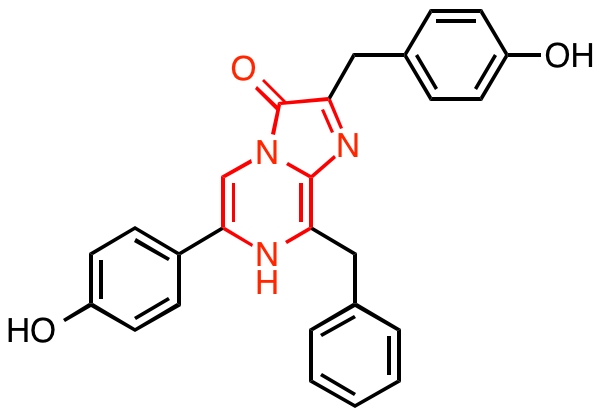
\includegraphics[width=0.8\textwidth]{coelenterazine.png}
\end{column}
\end{columns}
\end{frame}


\begin{frame}{Itemised Lists With Columns}
\begin{columns}[T]
\begin{column}{0.48\textwidth}
Lorem ipsum dolor sit amet, consetetur sadipscing elitr, sed diam nonumy eirmod tempor invidunt ut labore et dolore magna aliquyam erat, sed diam voluptua. At vero eos et accusam et justo duo dolores et ea rebum. Stet clita kasd gubergren, no sea takimata sanctus est Lorem ipsum dolor sit amet. Lorem ipsum dolor sit amet, consetetur sadipscing elitr, sed diam nonumy eirmod tempor.
\end{column}
\begin{column}{0.48\textwidth}
\begin{itemize}
   \item One point
   \item Another point
   \item And a \alert{third}!
   \item \textit{Four}?
\end{itemize}
\end{column}
\end{columns}
\end{frame}


\begin{frame}
\frametitle{Blocks}
\begin{block}{Blocks are Used for Emphasis in Beamer}
Anything can go in a block.
\begin{itemize}
   \item Bullet points.
   \item For demonstration,
   \item or to summarise something.
\end{itemize}
The box surrounding the title and content of a block will be the \texttt{themecolor} of the presentation.
\end{block}
\end{frame}


\begin{frame}
\frametitle{More Blocks}
\begin{alertblock}{This is an Alert Block}
Alert blocks are usually used for some key point to be highlighted in a talk.
A chemical reaction for example:\footnote{This example needs the \texttt{chemmacros} package, If you're writing about chemistry the author recommends it.}
\begin{equation}
   \ch{CH4 + 2 O2 -> 2 H2O + CO2}
\end{equation}

Alert blocks are red for all \texttt{themecolours} except the two reds. In those cases they're orange.
\end{alertblock}
\end{frame}


\begin{frame}
\frametitle{Even More Blocks}
\begin{exampleblock}{This is an Example Block}
The example block is usually used for examples. Here I find the solutions to a quadratic equation.
\begin{align*}
   2x^2 + 2x - 4 & = 0, \quad a=2, \quad b =2, \quad c=-4\\
   x & =\frac{-b\pm\sqrt{b^2-4ac}}{2a} \\
   x & =-2 \text{ or } 1
\end{align*}
Example blocks are dark green for all \texttt{themecolours} except the two greens. In those cases they're light blue.
\end{exampleblock}
\end{frame}


\section{The Legal Stuff}


\begin{frame}
The Beamer implementation 'UOWtheme' is copyright (CC BY-NC-SA 4.0 Int) 2015 by T. M. Griffiths under the \href{http://creativecommons.org/licenses/by-sa/4.0/}{Creative Commons Attribution-Share Alike 4.0 International License}\footnote{\url{http://creativecommons.org/licenses/by-nc-sa/4.0/}}.

\begin{center}\color{UOWdarkred}\ccbysa\end{center}

The crest and associated branding of the University of Wollongong is copyright and the property of the University of Wollongong. As the core identifier of the university its use is governed by the university's brand and visual identity guidelines which can be found \href{http://www.uow.edu.au/about/brand/uowlogo/index.html}{online}\footnote{\url{http://www.uow.edu.au/about/brand/uowlogo/index.html}}.

\end{frame}


\end{document}
